% 
% WebCrypto
% @author Pieter Maene <pieter.maene@student.kuleuven.be>
%

\chapter{Web Cryptography API}
\label{chap:web_cryptography_api}

Wanneer webontwikkelaars vandaag cryptografische functies nodig hebben in hun toepassingen, moeten ze bijna JavaScript gebruiken omwille van compatibiliteit. Hoewel er de laatste jaren zeer grote vooruitgang geboekt is, zullen de meeste JavaScript engines nog steeds minder goed presteren dan native code.\cite{site:resig_javascript_performance_rundown}\cite{site:cois_javascript_performance_rundown_2012}\cite{smedberg_performance_analysis_of_javascript} De W3C startte in 2012 een working group op om een nieuwe browser API te defini\"eren: de Web Cryptography API.\cite{wiki:webcrypto}

\npar In \ref{sec:wc:wb_cryptography_api} wordt deze nieuwe API kort besproken. Daarna wordt in \ref{sec:wc:nfwebcrypto} gekeken naar de NfWebCrypto polyfill, die de nieuwe functionaliteit implementeert in een plugin voor Google Chrome. Tot slot wordt deze implementatie in \ref{sec:wc:benchmarks} vergeleken met bestaande cryptografische libraries.

\section{Web Cryptography API~\cite{sleevi_watson_web_cryptography_api}}
\label{sec:wc:wb_cryptography_api}

De Web Cryptography API definieert cryptografische operaties die gebruik maken van sleutels die beheerd worden door de browser. Al deze methoden zitten in de \texttt{SubtleCrypto} interface. Er zijn zowel methodes voor het beheren van het sleutelmateriaal als het encrypteren van data. De laatste working draft op het moment van schrijven ondersteunt 21 cryptografische algoritmes. Het is wel zo dat niet elk algoritme alle methodes van de interface ondersteunt.

%TODO Meer Tekst

\section{NfWebCrypto}
\label{sec:wc:nfwebcrypto}

Aangezien de standaard nog niet voltooid was, werd deze nauwelijks ondersteund door de grote browsers.\cite{site:html5test_web_cryptography_api} Alleen Internet Explorer 11 had reeds een implementatie, maar hierin was slechts een beperkt aantal algoritmes aanwezig.\cite{site:microsoft_web_cryptography} Om de vergelijking met de andere JavaScript libraries toch te kunnen uitvoeren, was dus een implementatie nodig van deze API.

\npar PolyCrypt is een JavaScript polyfill ontwikkeld door BBN Technologies.\cite{site:polycrypt} Een polyfill implementeert een browser API die (nog) niet native ondersteund wordt. Omdat deze gebaseerd is op een oudere draft van de API, miste ook hierin functionaliteit die nodig was voor de tests. Een bijkomend nadeel aan deze implementatie is dat ze in JavaScript geschreven is, waardoor een eventueel snelheidsvoordeel ten opzichte van de andere libraries waarschijnlijk niet naar voor zou komen.

\npar NfWebCrypto daarentegen is een C\texttt{++} polyfill ontwikkeld door Netflix.\cite{site:nfwebcrypto} Intern wordt de bekende OpenSSL library gebruikt voor de cryptografische functionaliteit. Het grote voordeel is hier dus dat de cryptografische code nu native is, waardoor de prestaties vergelijkbaar zouden moeten zijn met die van een echte implementatie in de browser. Het grootste nadeel is hier wel dat het een plugin is voor Chrome. Bovendien moet deze handmatig gecompileerd worden en moet de browser op een speciale manier gestart worden, zodat het gebruik ervan niet zo vanzelfsprekend is. Hoewel dit dus gebruikt kan worden voor de tests, is dit niet direct bruikbaar voor praktische applicaties.

\section{Benchmarks}
\label{sec:wc:benchmarks}

\subsection{Modulaire exponentiatie}

\begin{figure}
  \center{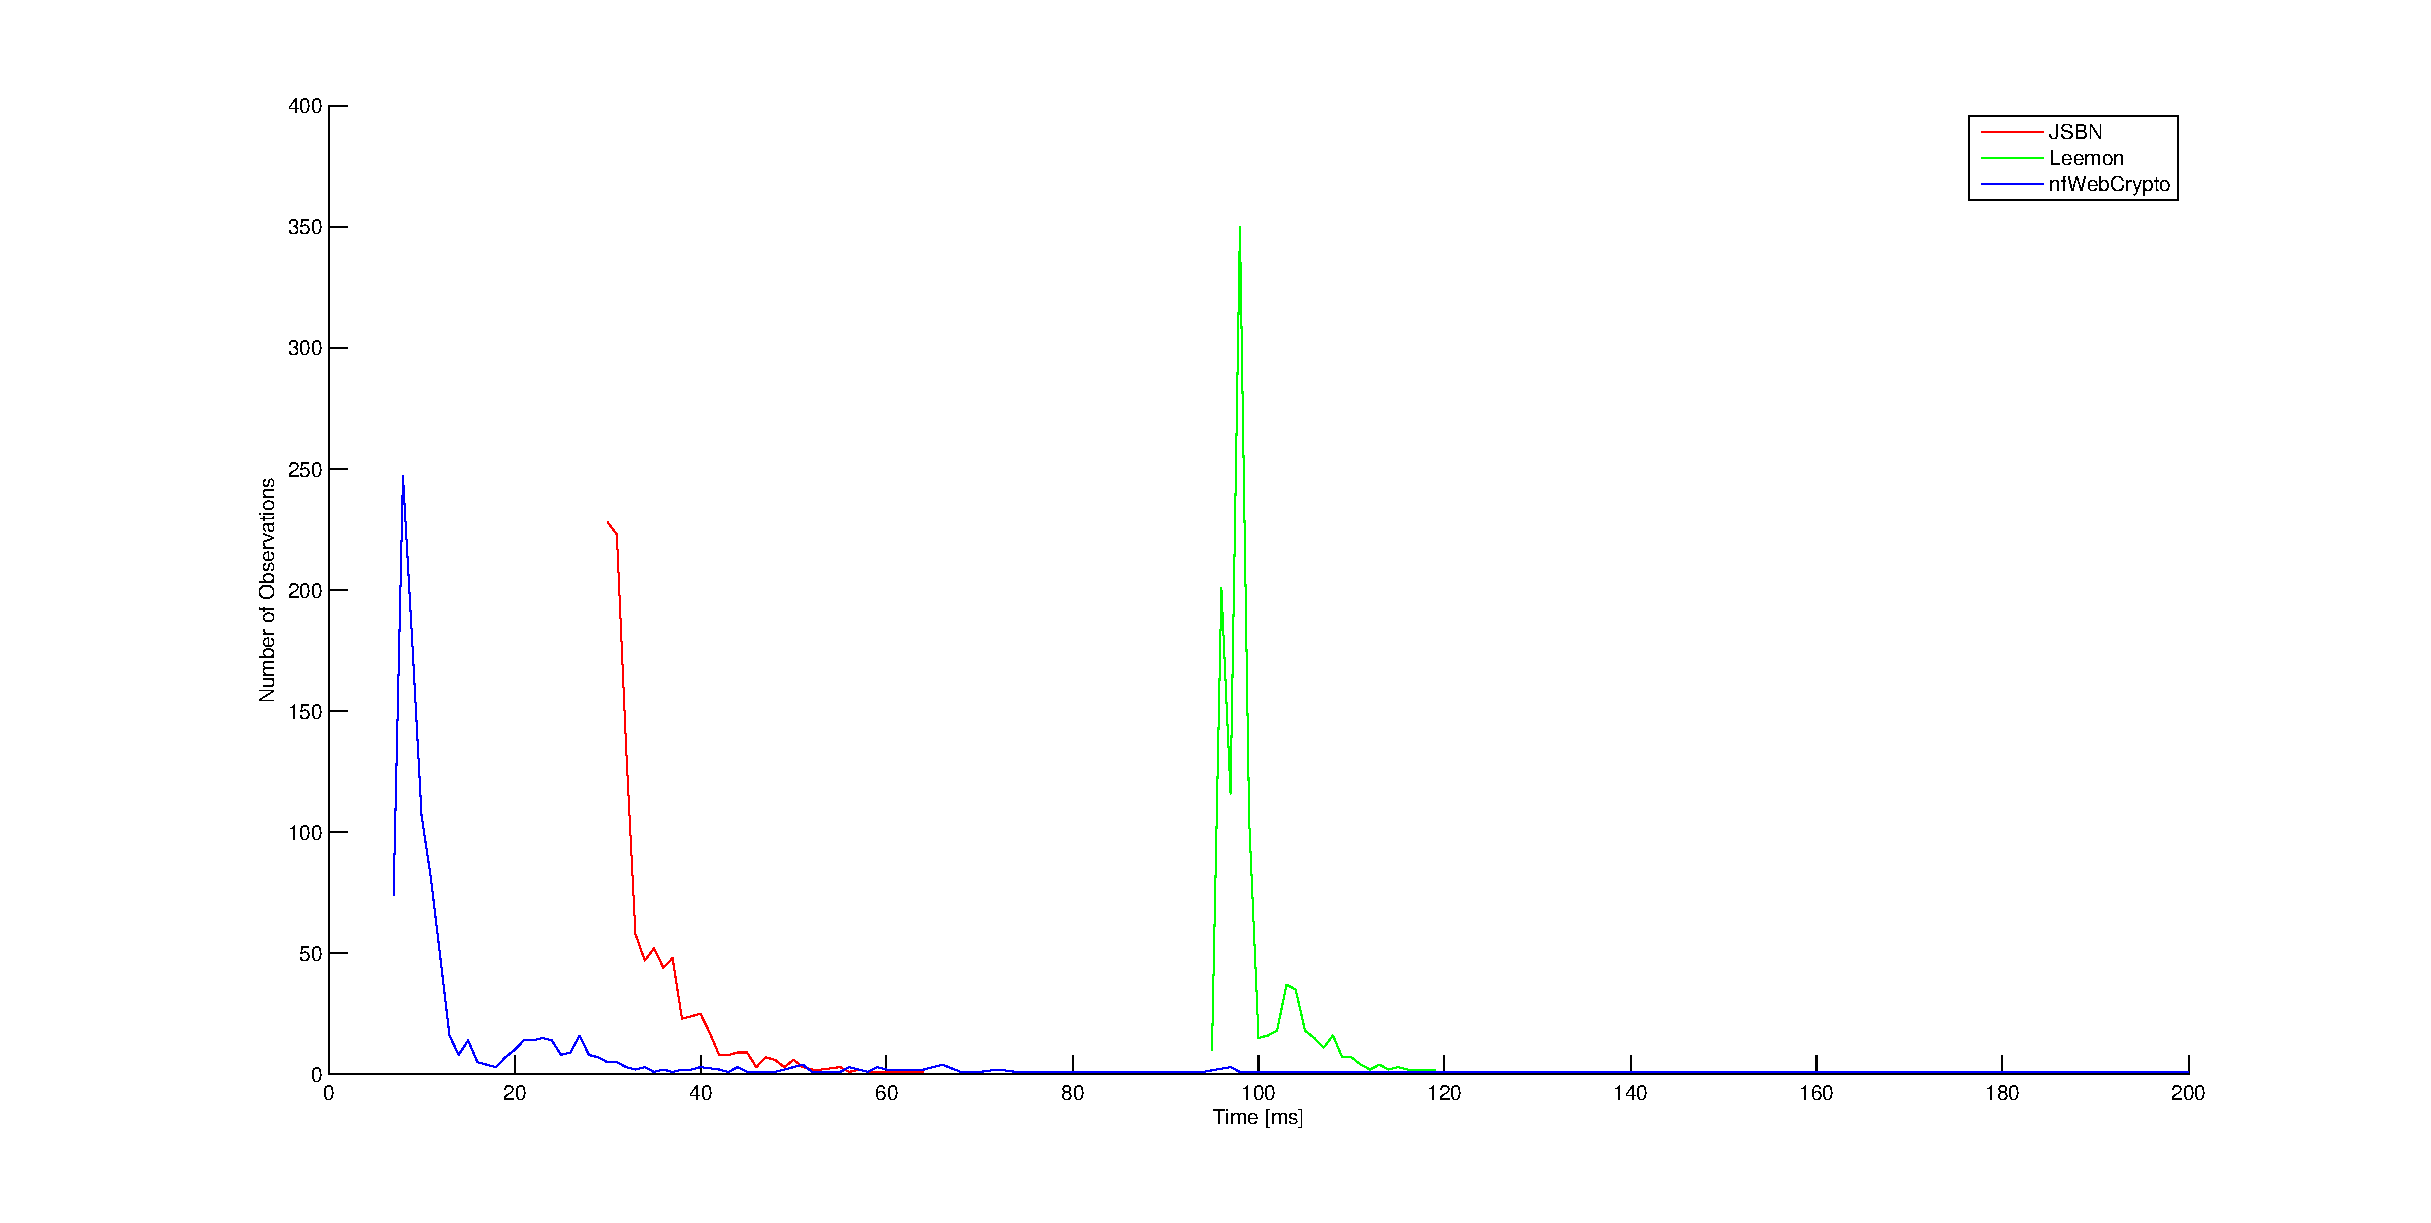
\includegraphics[width=\linewidth]{wc/modular_exponentiation.eps}}
  \caption{Modulaire exponentiatie}
  \label{fig:wc:modular_exponentiation}
\end{figure}

\begin{table}
  \begin{center}
    \begin{tabular}{r | c c}
      Library & Gemiddelde [ms] & Variantie [ms] \\ \hline
      JSBN & 33,9250 & 26,5019  \\
      Leemon & 99,1470 & 15,0785 \\
      NfWebCrypto & 16,0670 & 470,6251
    \end{tabular}
    \caption{Modulaire exponentiatie}
    \label{tab:wc:modular_exponentiation}
  \end{center}
\end{table}

\subsection{RSA}

\begin{figure}
  \center{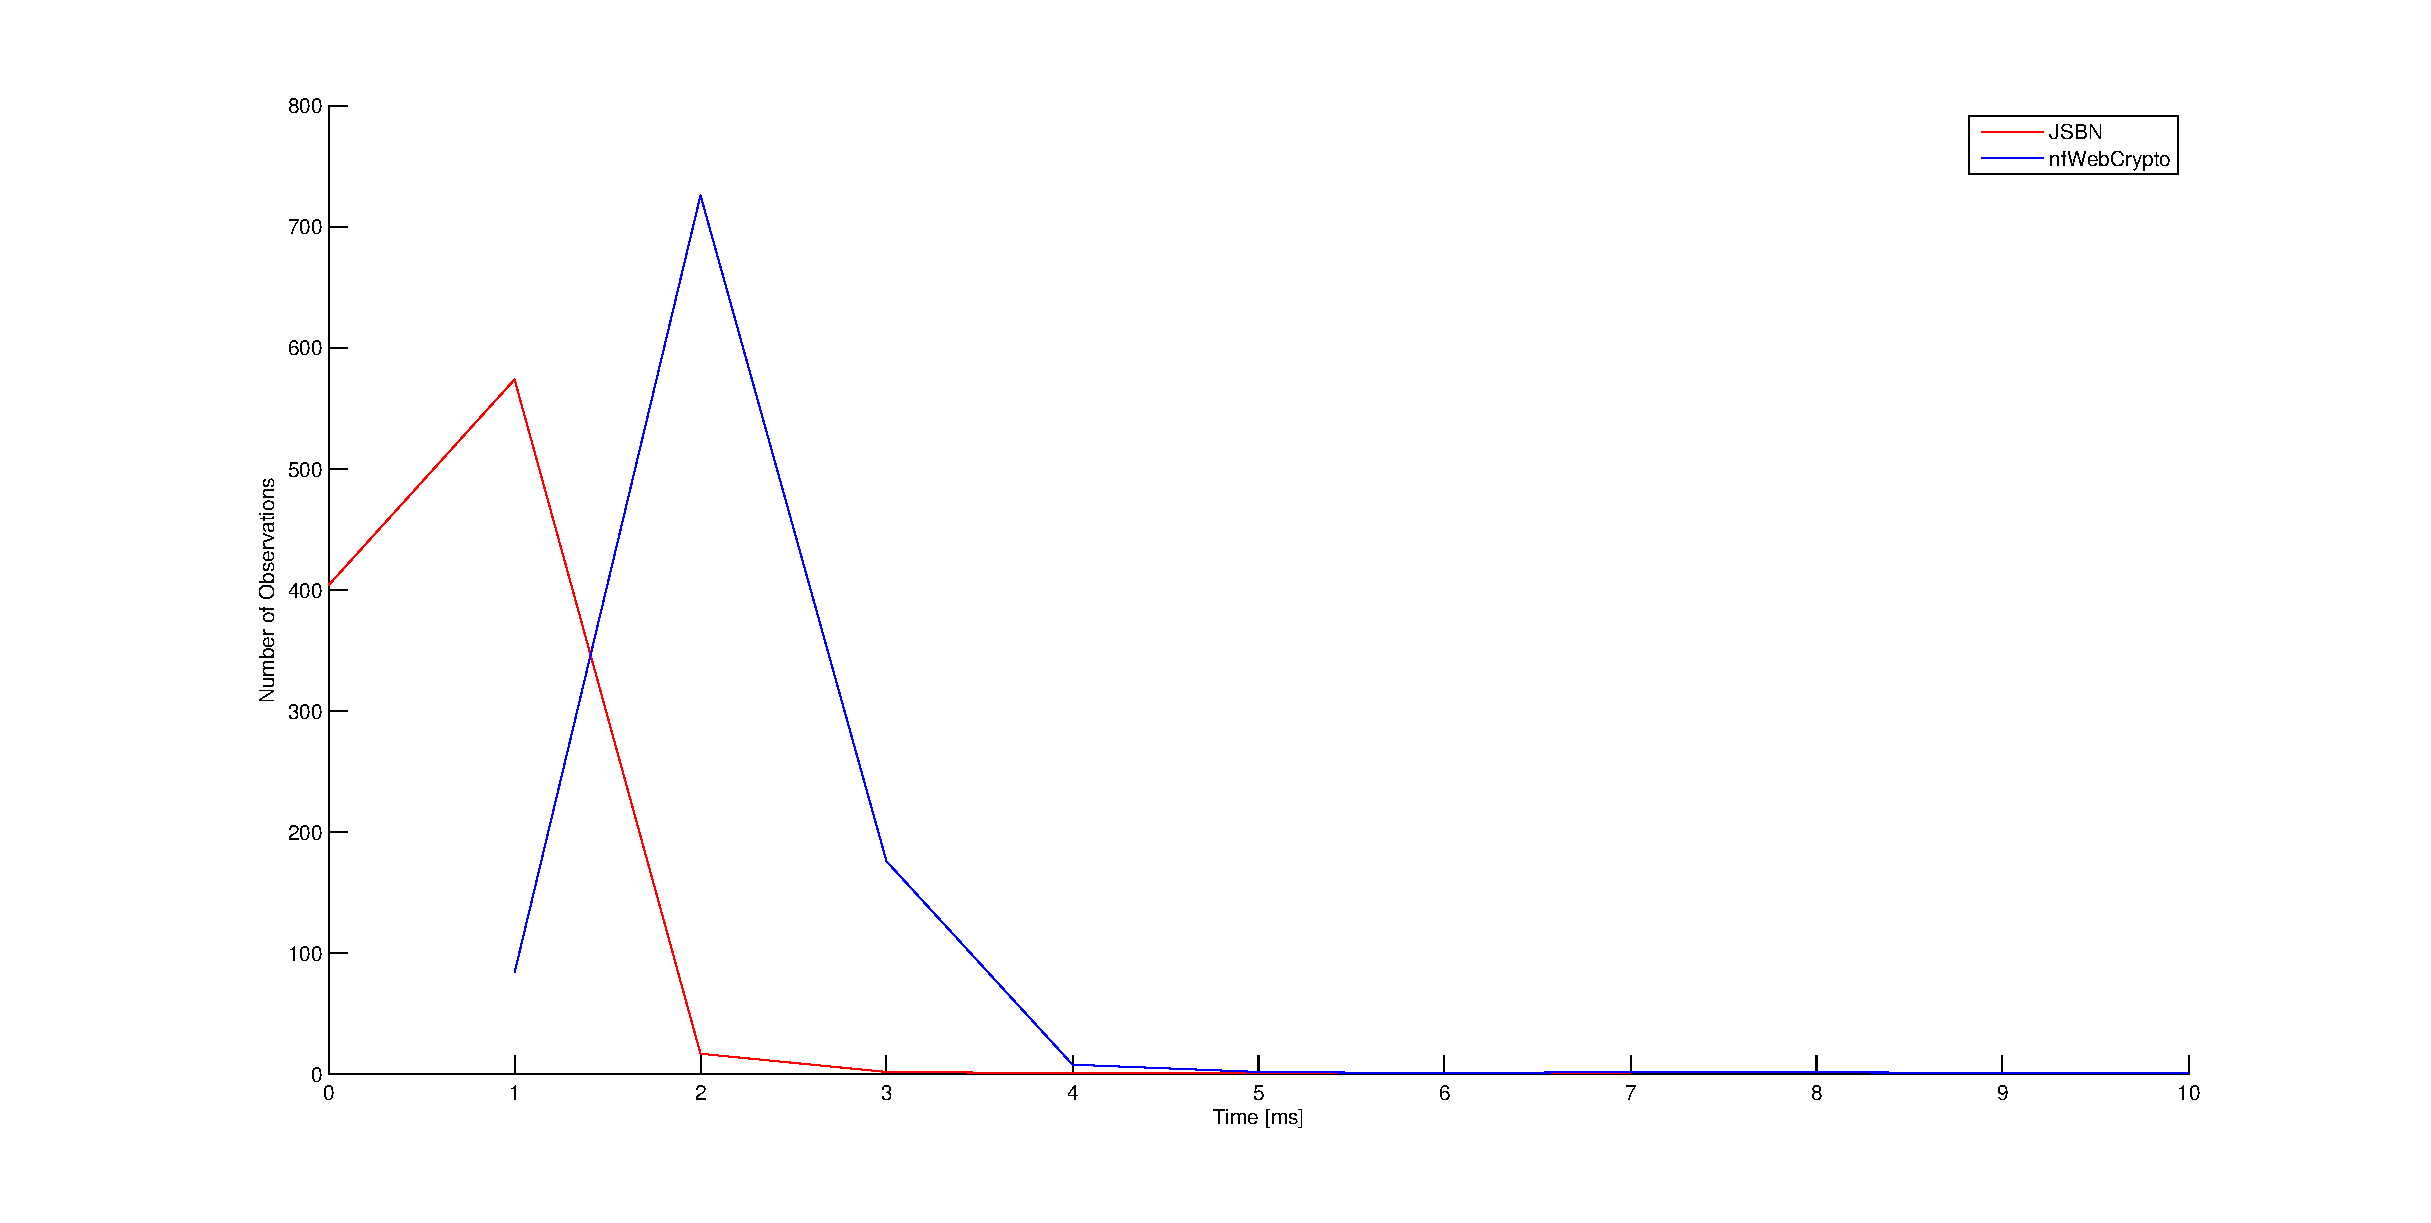
\includegraphics[width=\linewidth]{wc/rsa.eps}}
  \caption{RSA}
  \label{fig:wc:rsa}
\end{figure}

\begin{table}
  \begin{center}
    \begin{tabular}{r | c c}
      Library & Gemiddelde [ms] & Variantie [ms] \\ \hline
      JSBN & 0,6310 & 0,3632  \\
      NfWebCrypto & 2,1360 & 0,4219
    \end{tabular}
    \caption{RSA}
    \label{tab:wc:modular_exponentiation}
  \end{center}
\end{table}
